\section{Qualitative Reasoning}
\begin{itemize}
	\item Learning by making (qualitative) representations, combine meanings and reason with them
	\item Differs with numerical reasoning by not having exact values (we can express that something is positive, but we don't say it has the value $3.21$) 
\end{itemize}
\subsection{General vocabulary}
\begin{itemize}
	\item In QR, we express systems by the use of entities (like \textit{population}), and describe them by their quantities (e.g. \textit{size})
	\item We can define relations and inequalities between those. The full vocabulary is visualized in Figure~\ref{fig:kr_qr_vocabulary}
\end{itemize}
\begin{figure}[ht!]
	\centering
	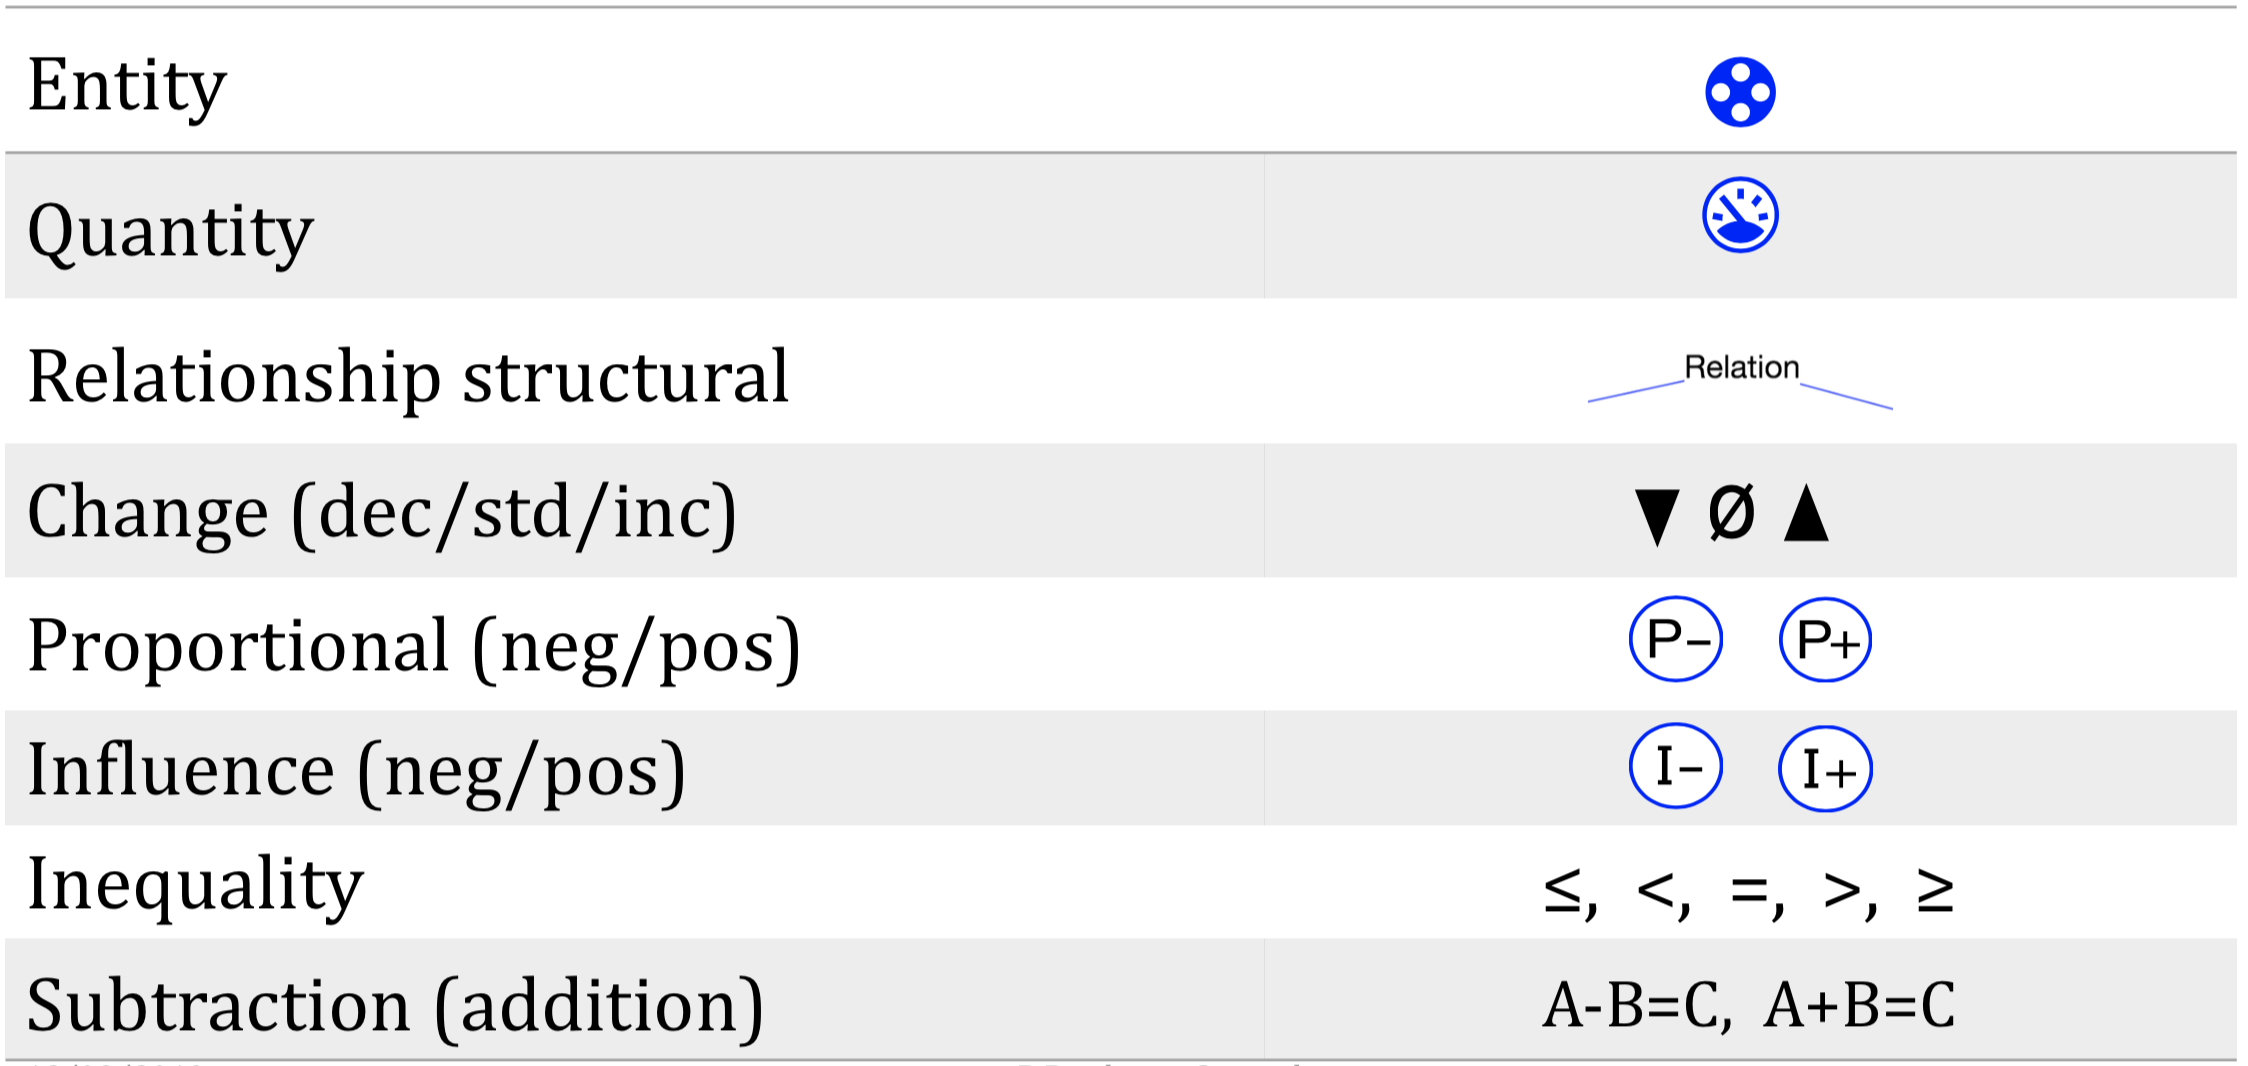
\includegraphics[width=0.45\textwidth]{figures/kr_qr_vocabulary.png}
	\caption{Overview of the vocabulary used in QR}
	\label{fig:kr_qr_vocabulary}
\end{figure}
\subsubsection{Quantities}
\begin{itemize}
	\item Quantities are described by a magnitude and a derivative (can also include higher order derivatives)
	\item The quantities are represented by a discrete scales which are build up by
	\begin{itemize}
		\item \textit{Intervals} which defines a range of values (e.g. $+$ for positive values)
		\item \textit{Landmarks} which reflect key points of the system, and are defined as single number (e.g. $0$ or $\max$)
	\end{itemize}
\end{itemize}
\subsubsection{Influence and Proportional}
\begin{itemize}
	\item \textbf{Proportional}: If \texttt{Q1} increases, then \texttt{Q2} increases (P+)/decreases (P$-$):
	$\partial \texttt{Q1}>0\implies \partial \texttt{Q2}>0$
	\begin{itemize}
		\item Mathematically, we can define the relation by:
		$$\texttt{Q2}\propto_{Q+}\texttt{Q1} \hspace{2mm}\equiv\hspace{2mm} \exists f\hspace{1mm}|\hspace{1mm}\texttt{Q2} = f(...,\texttt{Q1},...) \wedge f \text{ is increasing monotonic in }\texttt{Q1}$$
		\item This means that if \texttt{Q2} is \textit{qualitatively} proportional to \texttt{Q1}, we can express \texttt{Q2} by a function based on \texttt{Q1} such that it increases if \texttt{Q1} increases (and everything else stays the same)
		\item Monotonic functions provide an abstraction that cover a wide range of more mathematical expressions which can be narrowed by further constraints
	\end{itemize}
	\item \textbf{Influence}: If \texttt{Q1} is greater than 0, then \texttt{Q2} increases (I+)/decreases (I$-$):
	$\texttt{Q1} > 0\implies \partial \texttt{Q2}>0$
	\begin{itemize}
		\item Expressed in mathematical terms, the influence relation is stated as:
		$$I^{+}(\texttt{Q2},\texttt{Q1})\hspace{1mm} \equiv\hspace{1mm} d\texttt{Q2}/dt=...+B+...$$
		\item Note that this function definition is much more specific than for proportional. Hence it enables us knowledge of relative rates if multiple influences are given. Example: if $I^{+}(\texttt{Q2},\texttt{Q1})\wedge I^{-}(\texttt{Q2},\texttt{Q3})$, then we know that if $\texttt{Q1}>\texttt{Q3}$, $\texttt{Q2}$ increases.
		\item \textit{Warning}: for reasoning with influences, we often require the second-order derivative (if \texttt{Q1} has a derivative and doesn't change its qualitative magnitude, we can't model the change in the derivative of \texttt{Q2}). This is especially important if we have a positive and negative influence which both are in a interval with their magnitude.
	\end{itemize}
	\item Example in formulas:
	\begin{itemize}
		\item The change of the size of a closed population can be specified by:
		$N_{t+1} = N_{t} + B_{t} - D_{t}$
		where $B$ is the number of births, and $D$ the number of deaths between $t$ and $t+1$.
		\item Then, we have a positive influence of $B$ to $N$, and a negative influence of $D$ to $N$: $I^{+}(N,B)$, $I^{-}(N,D)$
		\item Further, we specify that the birth and death rate proportionally depend on the population size: $B=f_B(...,N,...)$, $D=f_D(...,N...)$ $\Rightarrow$ $P^{+}(D,N)$, $P^{+}(B,N)$
	\end{itemize}
	\item Both relations can lead to ambiguity if one influence/proportion is positive, and another is negative. Without given any other facts, all outcomes are possible new states
\end{itemize}
\subsubsection{Inequalities}
\begin{itemize}
	\item We can define inequalities between quantities (magnitudes), landmarks and derivatives
	\item Inequalities state a rather uncertain knowledge, or assumptions that are valid for at least the initial state
	 \item For example, we can state that $A$ is larger than $B$, but this might change during the simulation
	 \item Also, we can reason with inequalities by propagating knowledge (if $A>B$ and $B>C$, then $A>C$). This can for example lead to constraints in the value space of another quantity
\end{itemize}
\subsubsection{Value constraint}
\begin{itemize}
	\item The value constraint binds landmarks/intervals of two quantities together.
	\item If we have a value constraint from $A$ to $B$ to both 0, this means that if $A=0$ then $B=0$ (directed relation!)
\end{itemize}
\subsection{States and Transitions}
\begin{itemize}
	\item A qualitative state is a period of time in which the qualitative behavior of the system doesn't change (changes include magnitudes, derivatives, inequalities, etc.)
	\item Thus, states are \textit{unique} sets of inequality quantity expressions
	\item Transitions are changes of at least one quantity (but all changes must take place to enter the next state if multiple quantities change)
\end{itemize}
\begin{figure}[ht!]
	\centering
	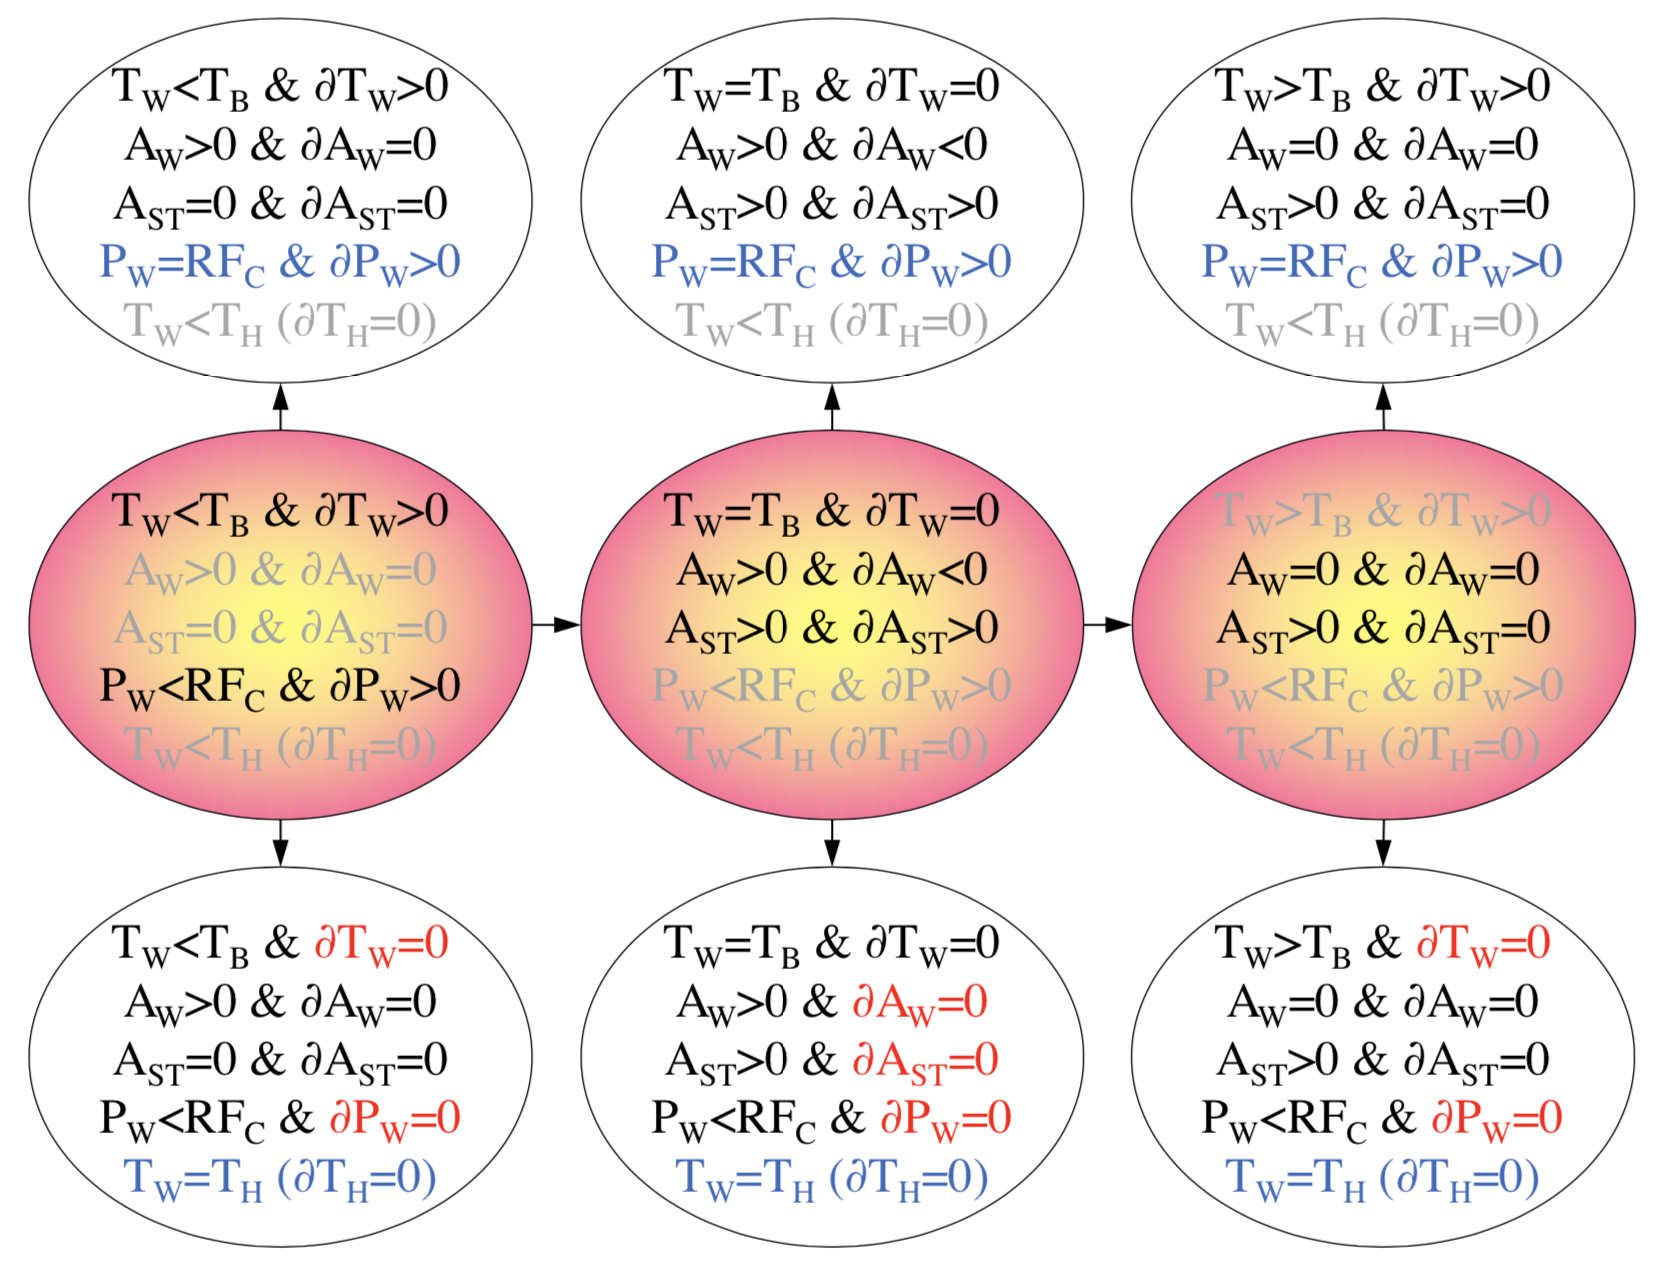
\includegraphics[width=0.5\textwidth]{figures/kr_qr_state_graph_example.png}
	\caption{Example state graph for heating water in a cattle}
	\label{fig:kr_qr_state_graph_example}
\end{figure}
\subsubsection{Compositional modeling}
\begin{itemize}
	\item To improve re-usability of QR definitions, we can split the model into several parts
	\item We define a hierarchy of generic entities (e.g. population) on which we will operate
	\item The library of model fragments contain structures that defines certain entities/quantities and their relation (if a population exists, then...). These can be conditioned on assumptions (e.g. closed or open population)
	\item In the scenarios, we define certain instances of our entity hierarchy (e.g. ``\textit{Green Frogs}'' as instance of entity population). Based on them, we can state initial values (e.g. population size is max), and assumptions we make (e.g. closed population)
	\item We then combine both the scenario and the model fragment to create the behavior graph
\end{itemize}
\begin{figure}[ht!]
	\centering
	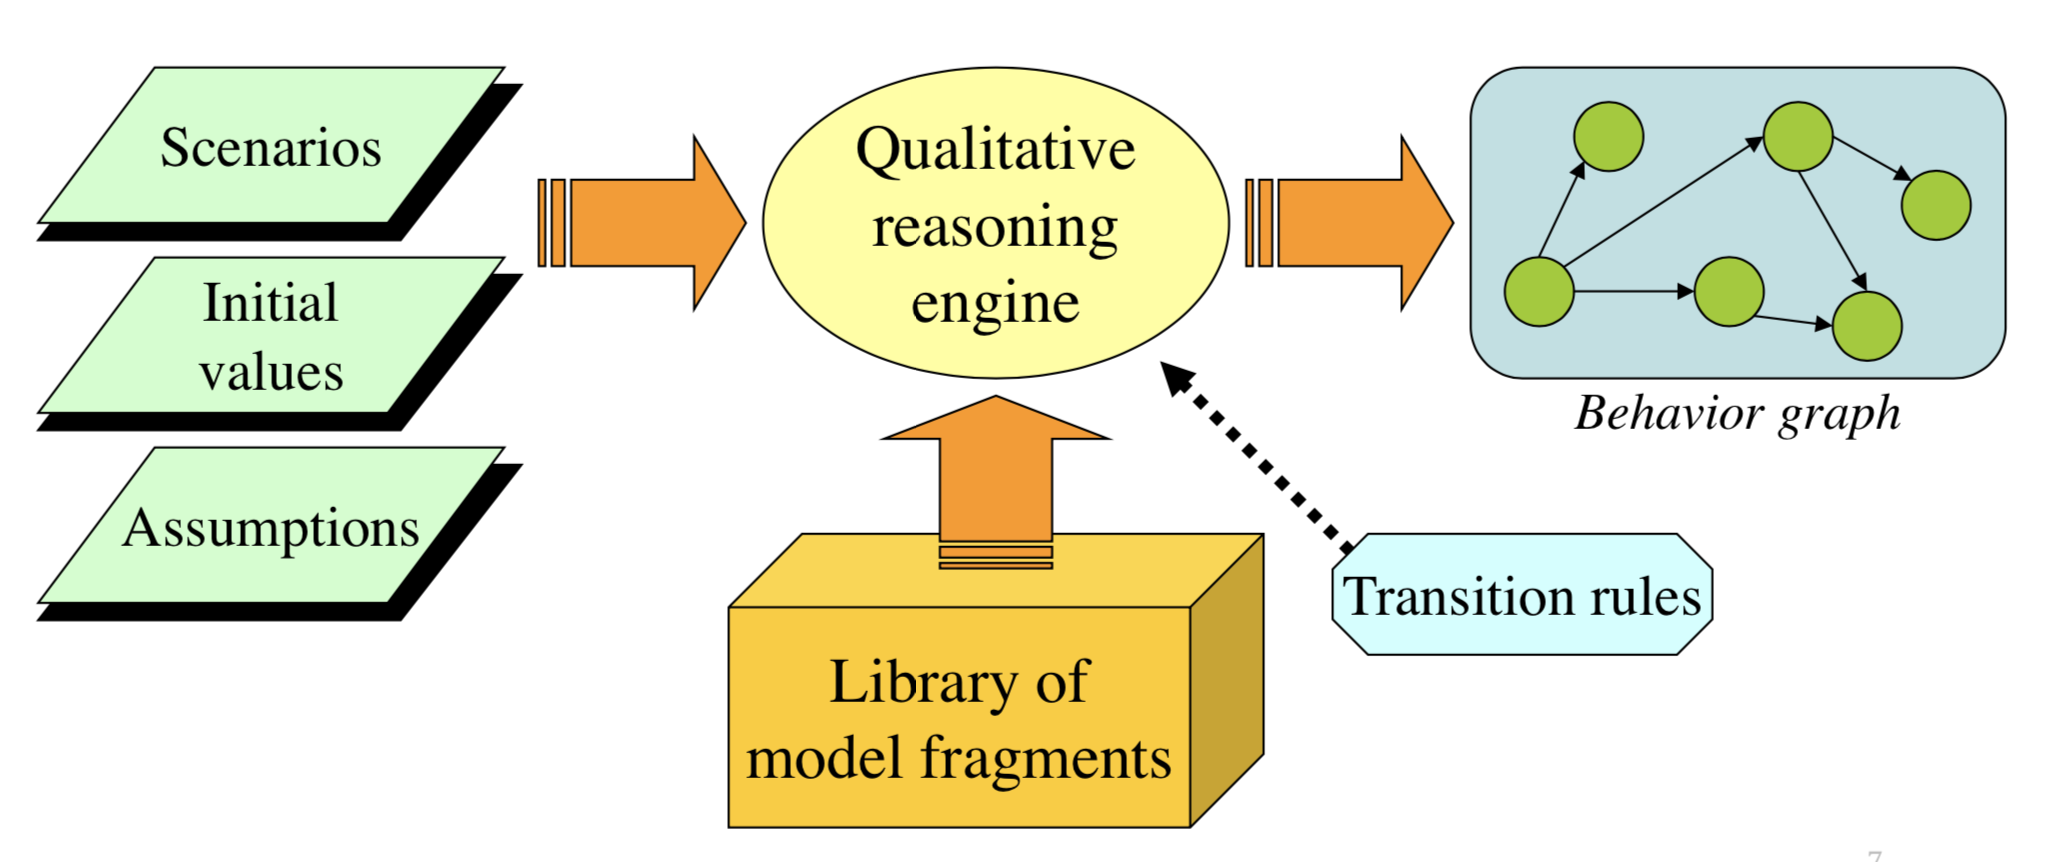
\includegraphics[width=0.5\textwidth]{figures/kr_qr_compositional_modeling.png}
	\caption{Compositional modeling}
	\label{fig:kr_qr_compositional_modeling}
\end{figure}
\subsubsection{Finding transitions}
\begin{itemize}
	\item There are three common types of termination 
	\begin{itemize}
		\item \textbf{Value termination}: if a quantity has a derivative in a certain direction, then it can move to the next quantity point in this direction
		\item \textbf{Inequality termination}: Given a inequality, if one side is changing due to derivatives, then the truth value might change (from $\texttt{Q2}>\texttt{Q1}$ to $\texttt{Q2}=\texttt{Q1}$, remember continuous changes!)
		\item \textbf{Exogenous termination}: An external effect/input that leads to a change. Can for example be controlling the derivative of a quantity. The behavior can be random, sinusoidal, random, etc.
	\end{itemize}
	\item Another important concept for deciding on transitions is \textbf{Epsilon ordering} dealing with value termination
	\begin{itemize}
		\item We distinguish between \textit{immediate} and \textit{non-immediate} transitions
		\item Immediate transitions are if a derivative is unequals 0 and the magnitude is currently at a landmark/point. Then, we will immediately move to the next state with the magnitude being changed
		\item Non-immediate transitions are when the derivative is unequals zero, but the magnitude is in an interval. Then it can change at some point, but does not have to be
	\end{itemize}
	\item Another concept we have to consider is value correspondence
	\begin{itemize}
		\item If two values are restraint by a value correspondence, then this can limit the possible transitions we can have
		\item For example, in Figure~\ref{fig:kr_qr_value_correspondence_termination}, we can either apply \texttt{T1} or \texttt{T2}, but both can't happen at the same time because then the value correspondence is not fulfilled
		\begin{figure}[ht!]
			\centering
			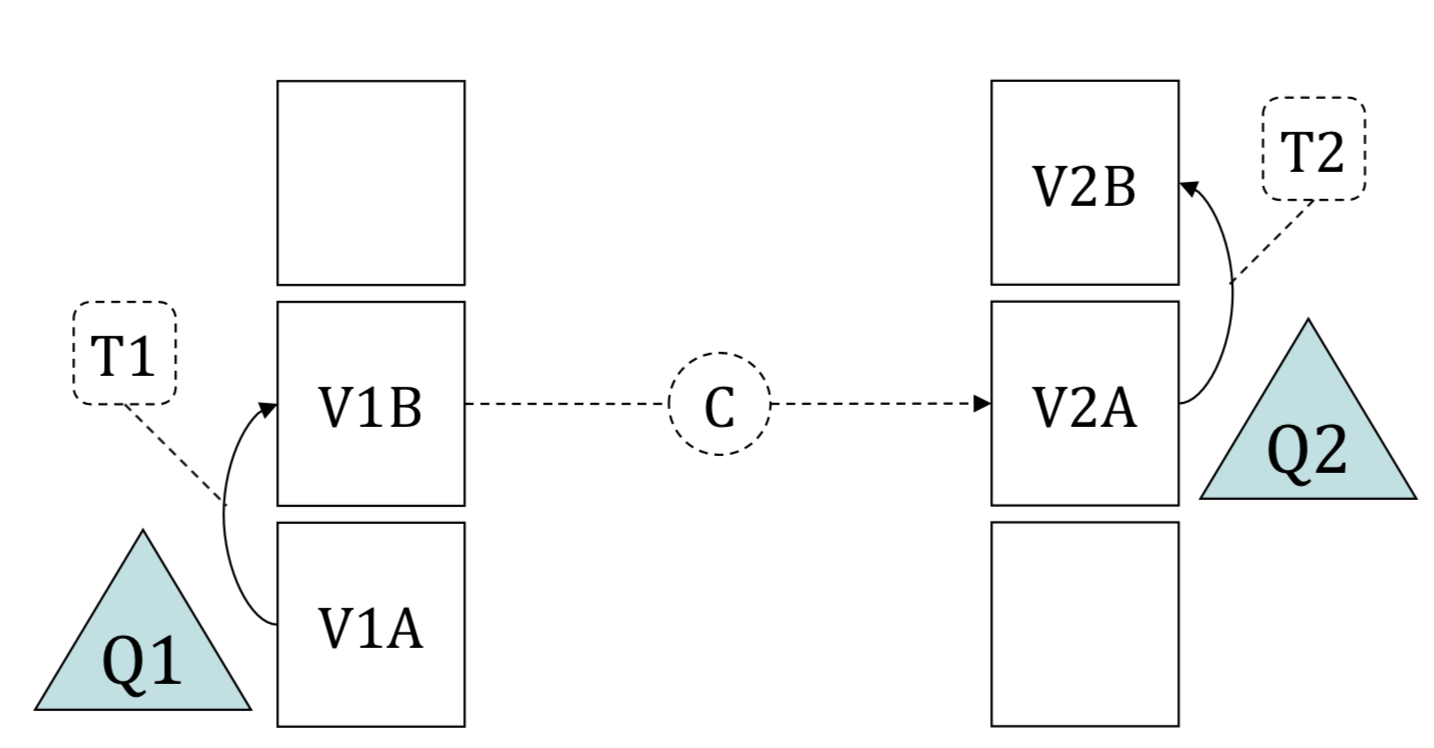
\includegraphics[width=0.4\textwidth]{figures/kr_qr_value_correspondence_termination.png}
			\caption{Example for transitions that exclude each other because of a value constraint}
			\label{fig:kr_qr_value_correspondence_termination}
		\end{figure}
	\end{itemize}
\end{itemize}